% Драфт: секция 2.3 — Восстановление геометрии среды из популяционной активности нейронов гиппокампа
% Источник: Sotskov2022 (IJMS)
% Куда: part2.tex, секция \ref{sec:geometry}

\section{Восстановление геометрии среды из популяционной активности нейронов гиппокампа}\label{sec:geometry}

В данном разделе описывается применение метода лапласовых собственных карт (LE, см.\ раздел~\ref{sec:dimred_methods}) к данным кальциевого имиджинга нейронов гиппокампа мышей, свободно исследующих O-образный трек~\cite{Sotskov2022}. Показано, что нелинейное снижение размерности позволяет восстановить геометрию среды непосредственно из многомерной нейронной активности, без использования информации о положении животного.

\subsection{Минископная регистрация нейронной активности при свободном исследовании кругового трека}

Девять мышей C57BL/6J (возраст 2--3 мес.) с экспрессией одного из генетически кодируемых кальциевых индикаторов (GCaMP6s, GCaMP7f, NCaMP7, FGCaMP7) в поле CA1 гиппокампа были имплантированы GRIN-линзой диаметром 1~мм. Для регистрации нейронной активности использовался минископ NVista HD (Inscopix) с частотой кадров 20~Гц. В каждой сессии мышь помещалась на 15~мин в приподнятый O-образный трек (диаметр 50~см, ширина 5~см, высота бортиков 5~см) с проксимальными (различный материал бортов) и дистальными (метки на шторе) визуальными ориентирами. Мыши свободно исследовали среду без какого-либо подкрепления, совершая в среднем 19 кругов за сессию. Для 8 из 9 мышей сессия повторялась через 24~ч, для 3 мышей~--- через 48~ч.

Обработка данных кальциевого имиджинга (коррекция движения, экстракция нейронных компонент, детекция кальциевых событий) проводилась в соответствии с общим конвейером, описанным в разделе~\ref{sec:calcium_methods}. Совмещение нейронов между сессиями выполнялось с помощью CellReg~\cite{Sheintuch2017}.

\subsection{Детекция клеток места}

Для выявления пространственно-селективных нейронов использовался консервативный подход, учитывающий как пространственную, так и временн\'{у}ю устойчивость активности~\cite{Sotskov2022}. Пространство трека разделялось на 20 секторных бинов размером $5 \times 7{,}5$~см. Для каждого нейрона подсчитывалось пространственное распределение кальциевых событий, которое сглаживалось гауссовым ядром и пороговалось для выделения кандидатов в рецептивные поля.

Для оценки временн\'{о}й устойчивости вычислялся показатель селективности (selectivity score)~--- отношение числа кальциевых событий нейрона в пределах рецептивного поля к общему числу событий при данном и смежных посещениях. Нейрон считался клеткой места при наличии не менее трёх последовательных посещений рецептивного поля с показателем селективности выше 0{,}5. Латентность настройки (tuning latency) определялась как число посещений до начала первой устойчивой последовательности.

В первый день 25{,}1\% рецептивных полей формировалось при первом же посещении; средняя латентность настройки составляла 7 посещений (247~с). Во второй день латентность значимо снижалась ($p = 0{,}049$, двухфакторный дисперсионный анализ), при этом кумуляции показателя селективности между днями не наблюдалось. Данная динамика свидетельствует о том, что ускорение формирования пространственного кода в знакомой среде обусловлено популяционными механизмами, а не увеличением селективности отдельных нейронов.

\subsection{Снижение размерности нейронной активности методом лапласовых собственных карт}

Для популяционного анализа данные кальциевой активности представлялись в виде матрицы $D_{N \times T}$, где $N$~--- число нейронов, $T$~--- длина записи в кадрах, и каждый столбец $\mathbf{v}_t \in \mathbb{R}^N$ задавал вектор активности популяции в момент~$t$. Учитывались только нейроны с 5 и более кальциевыми событиями за сессию. Временн\'{ы}е ряды предварительно усреднялись скользящим окном шириной 8 кадров (0{,}4~с), что не влияло качественно на результаты.

По полученным $T_{\text{eff}} = T/w$ точкам в $\mathbb{R}^N$ строился граф $k$ ближайших соседей ($k$-БС) на основе евклидова расстояния. Параметр $k$ выбирался минимальным, обеспечивающим связность графа: при малых $k$ соблюдается допущение локальной линейности многообразия, необходимое для корректной работы метода. Матрица смежности симметризовалась для получения ненаправленного графа.

Далее применялся метод LE (подробное описание~--- в разделе~\ref{sec:dimred_methods}): для графового лапласиана $L = D_{\text{deg}} - A$ решалась обобщённая задача на собственные значения $L\mathbf{u} = \lambda D_{\text{deg}}\mathbf{u}$, где $D_{\text{deg}}$~--- матрица степеней, $A$~--- матрица смежности. Первые два нетривиальных собственных вектора (после отбрасывания тривиального $\lambda_0 = 0$) задавали двумерное вложение графа.

Для количественной оценки качества восстановления геометрии трека использовалась метрика остаточной дисперсии (residual variance, RV)~\cite{tenenbaum2000}:
\begin{equation*}
    RV = 1 - \rho^2(D_h, D_l),
\end{equation*}
где $\rho$~--- коэффициент корреляции Пирсона между матрицами попарных евклидовых расстояний в пространстве реальных координат мыши ($D_h$) и в пространстве вложения ($D_l$). RV принимает значения от 0 (точное восстановление) до 1.

\subsection{Восстановление геометрии трека из нейронной активности}

Метод LE был применён к данным шести мышей с достаточным числом зарегистрированных нейронов ($N > 200$) в первый день записи. Первые две компоненты вложения совпали с координатами мыши на треке с точностью до поворота на фиксированный угол (рис.~\ref{fig:sotskov5}). Алгоритм не получал никакой информации о реальном положении животного~--- геометрия трека извлекалась исключительно из коллективной динамики нейронов.

Воспроизвести этот результат с помощью метода главных компонент (PCA) не удалось: первые две главные компоненты не обнаруживали кольцевой структуры (рис.~\ref{fig:sotskov5}C), что указывает на нелинейный характер связи между нейронной активностью и пространственными координатами.

\begin{figure}[ht]
    \centering
    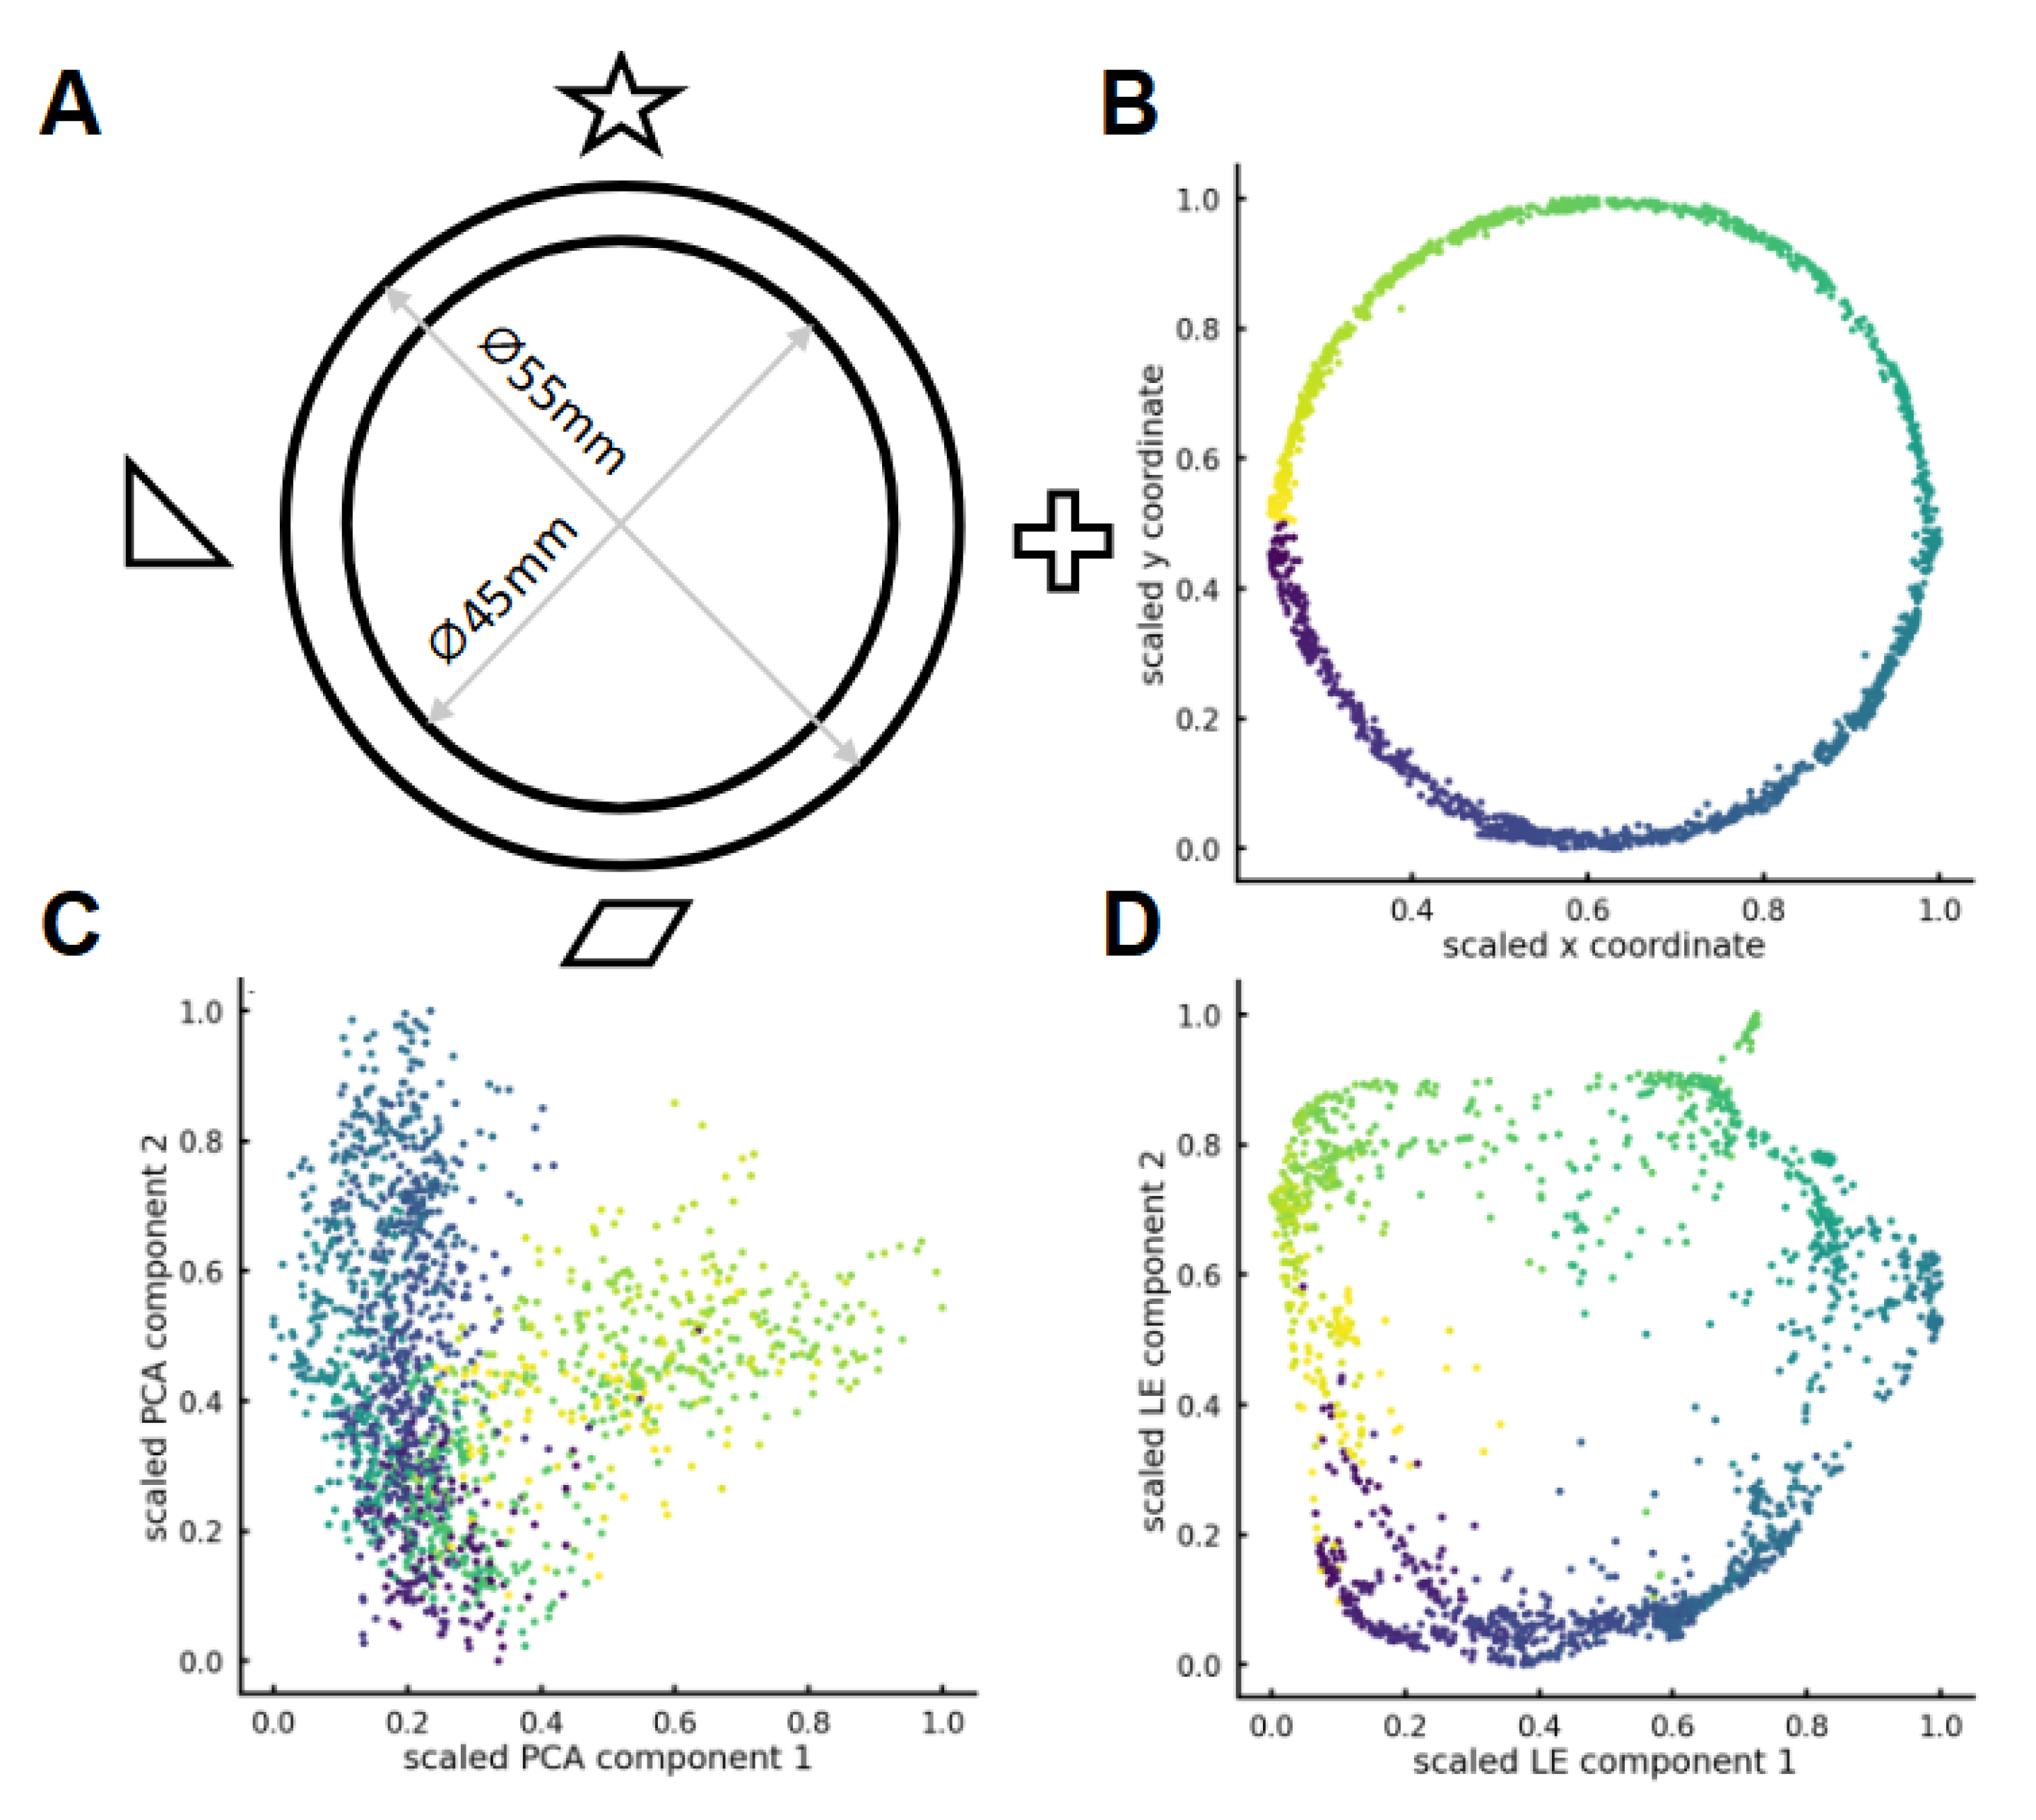
\includegraphics[width=0.85\textwidth]{images/sotskov/fig5.png}
    \caption{Восстановление геометрии O-образного трека из активности CA1. (\textbf{A})~Круговой трек с визуальными ориентирами. (\textbf{B})~Поточечное представление траектории. (\textbf{C})~Первые две оси PCA-вложения. (\textbf{D})~Первые две оси LE-вложения (собственные векторы графового лапласиана). Адаптировано из~\cite{Sotskov2022}.}
    \label{fig:sotskov5}
\end{figure}

\subsection{Зависимость качества восстановления от размера популяции и времени записи}

Остаточная дисперсия вложения убывала с увеличением числа зарегистрированных нейронов (рис.~\ref{fig:sotskov6}C), что свидетельствует о распределённом характере пространственного кода: нелинейное снижение размерности позволяет выделить популяционные переменные, которые невозможно извлечь из активности малого числа клеток.

Кроме того, остаточная дисперсия убывала по ходу сессии (рис.~\ref{fig:sotskov6}B): по мере знакомства мыши со средой качество восстановления геометрии улучшалось. Этот эффект был тем сильнее, чем больше нейронов было зарегистрировано у данного животного.

Для сопоставления популяционной и индивидуальной мер пространственного кодирования сравнивались средний показатель селективности и средняя ошибка восстановления для каждой мыши. Распределения этих двух величин показали косинусное сходство $0{,}968 \pm 0{,}047$ (рис.~\ref{fig:sotskov6}D), что подтверждает согласованность популяционного и поклеточного подходов к оценке качества пространственного кодирования.

\begin{figure}[ht]
    \centering
    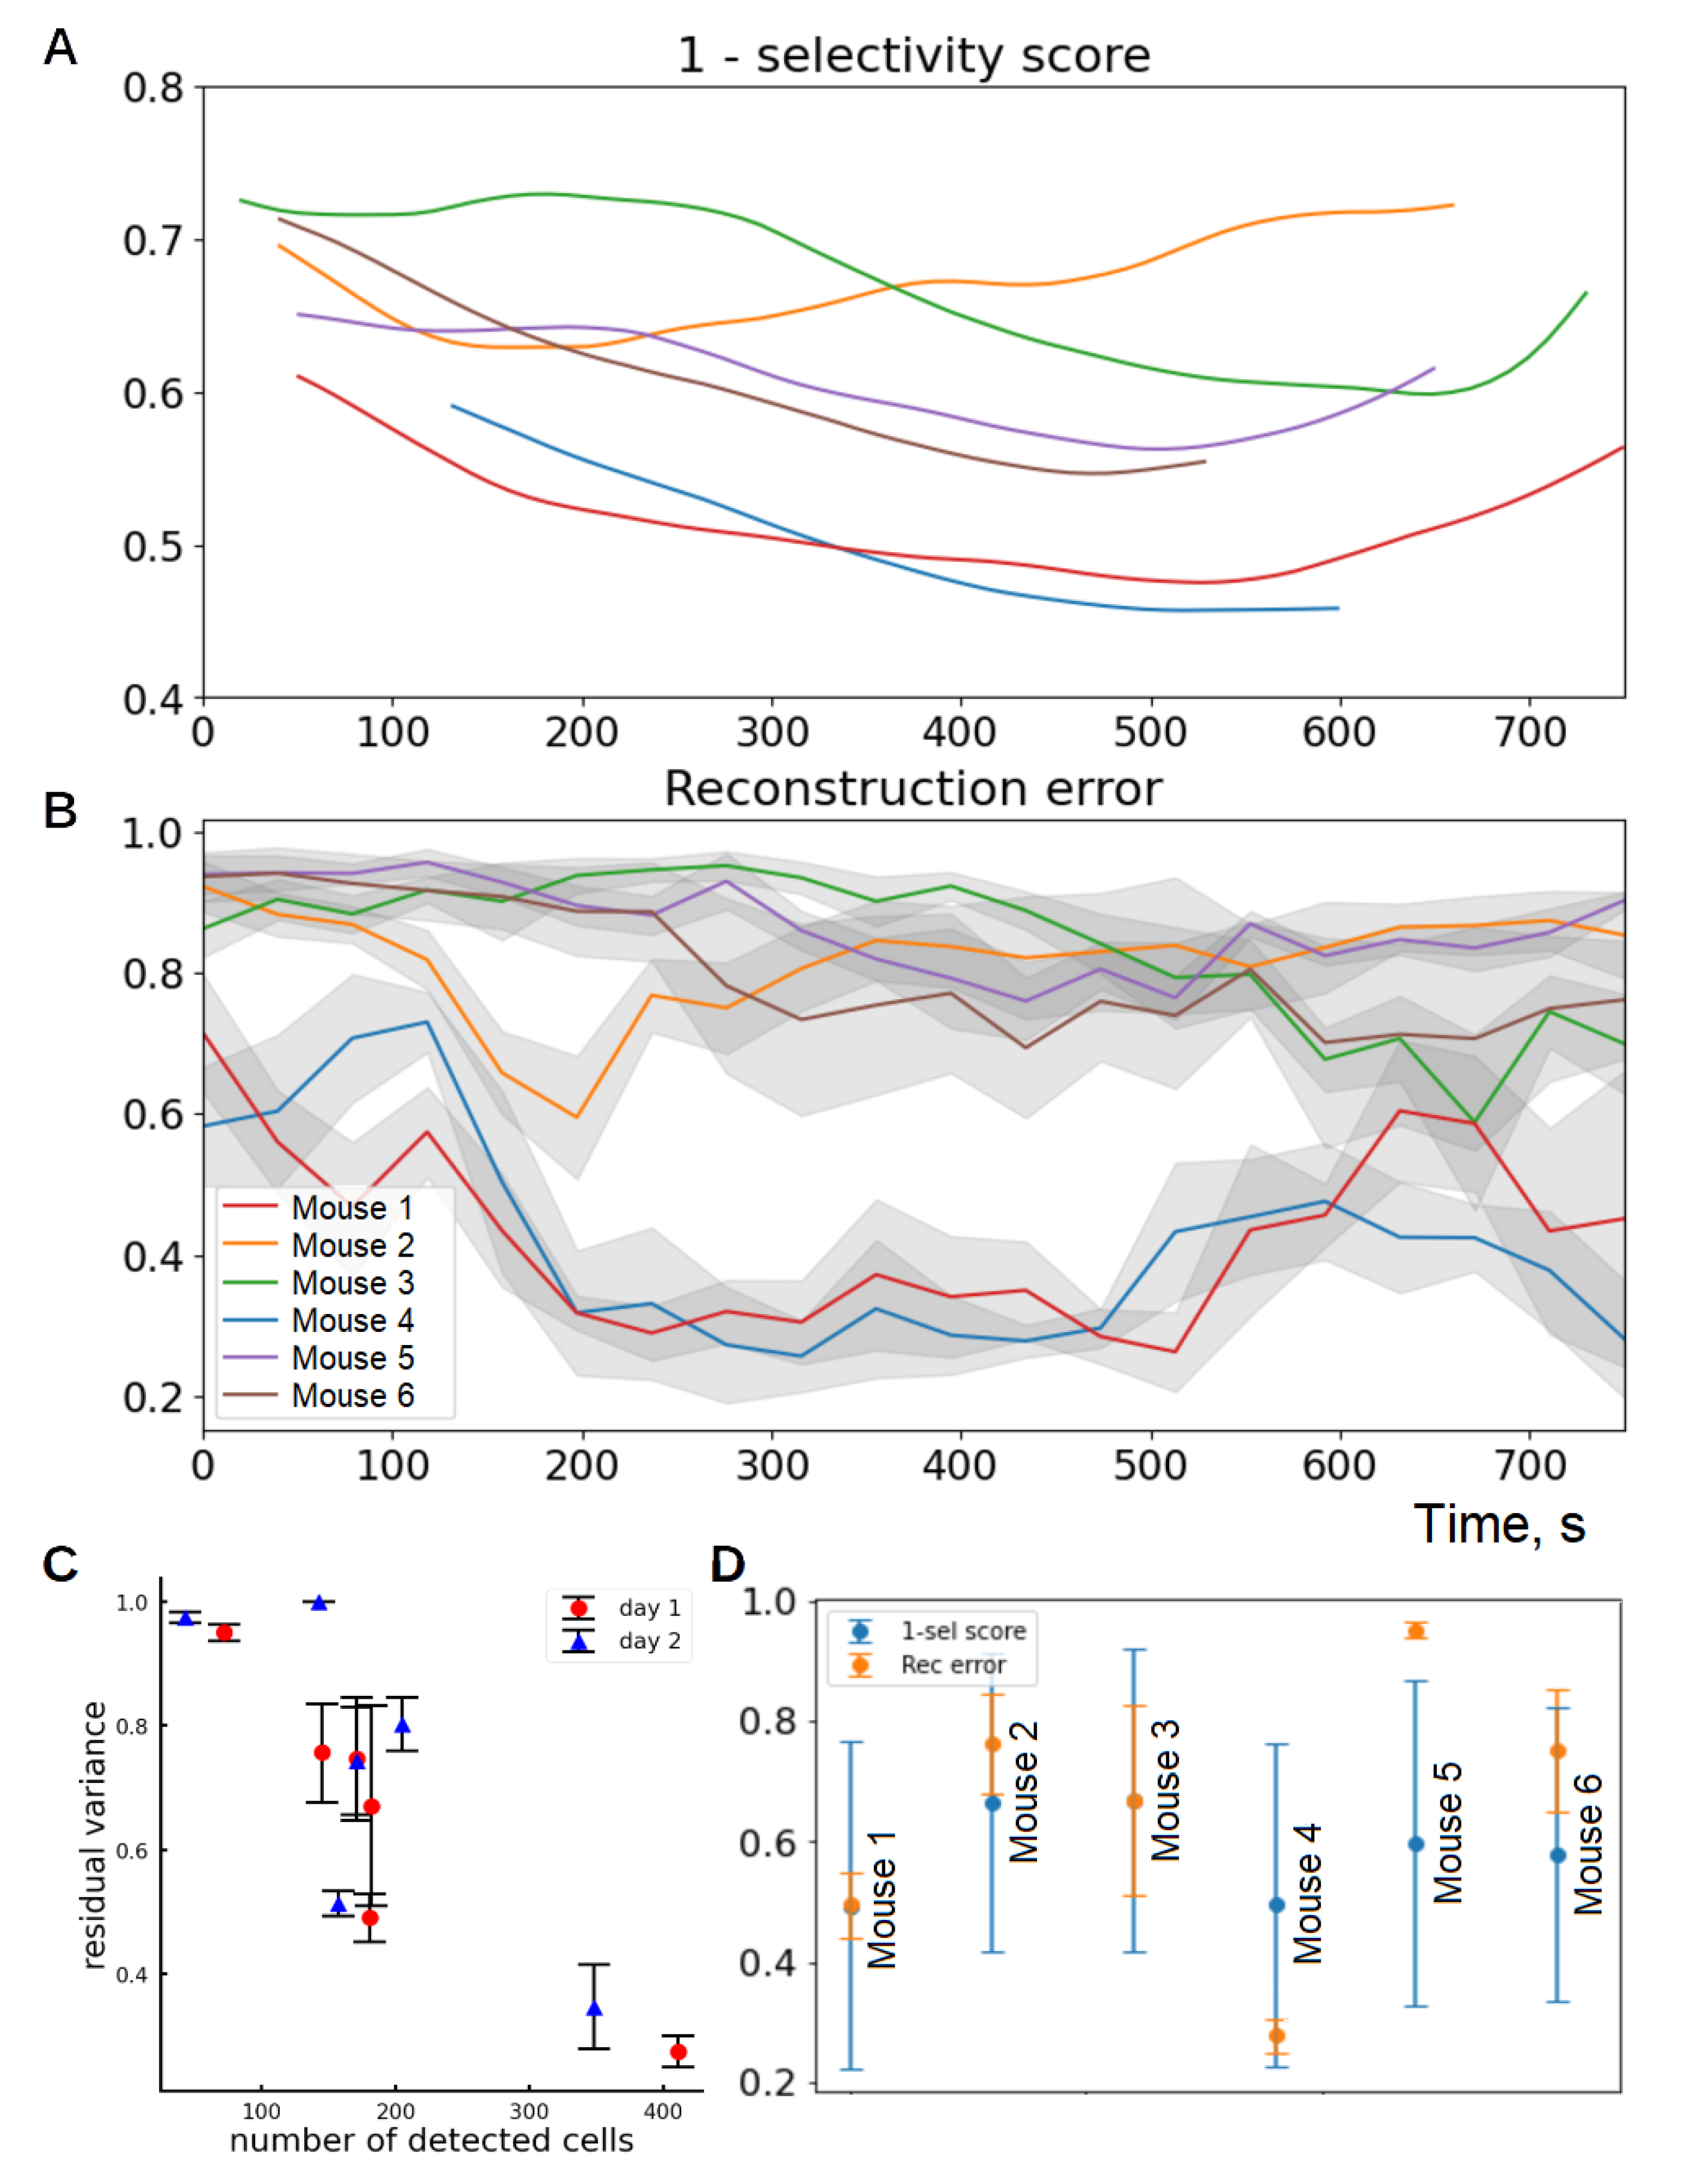
\includegraphics[width=0.85\textwidth]{images/sotskov/fig6.png}
    \caption{Качество восстановления геометрии трека. (\textbf{A})~Инвертированный средний показатель селективности (unselectivity score), интерполированный и сглаженный скользящим средним (окно 250~с). (\textbf{B})~Эволюция остаточной дисперсии (RV) в течение первой сессии; снижение размерности выполнялось для скользящего временн\'{о}го окна длиной 250~с; NC~--- число зарегистрированных нейронов. (\textbf{C})~Зависимость RV от числа зарегистрированных нейронов. (\textbf{D})~Средние показатели <<неселективности>> и ошибки восстановления по мышам; косинусное сходство $0{,}968 \pm 0{,}047$. Адаптировано из~\cite{Sotskov2022}.}
    \label{fig:sotskov6}
\end{figure}

Полученные результаты демонстрируют, что коллективная активность популяции нейронов CA1 содержит информацию о геометрии среды и что эта информация доступна для извлечения методами нелинейного снижения размерности. При этом линейные методы (PCA) не справляются с данной задачей, что подчёркивает нелинейный характер нейронного многообразия~--- в согласии с результатами анализа внутренней размерности, представленными в разделе~\ref{sec:dim}.
